% !TeX root = ../main.tex
\section{Approach and Training}
\label{sec:training}
The system couples three learned decisions through the physical continuation
they induce. Figure~\ref{fig:system} separates the episode's forward flow from
the supervision that connects G, P, and I.
\ifshowfigures
\begin{figure}[H]
\centering
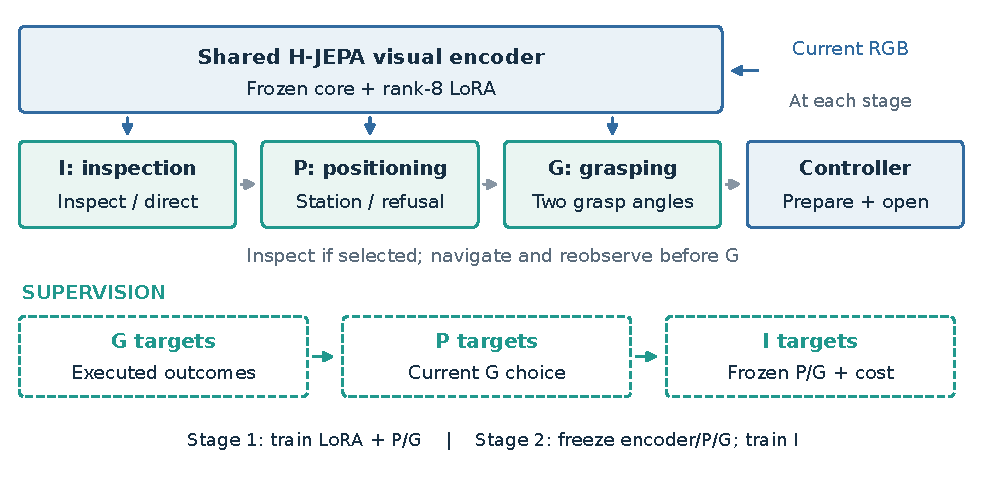
\includegraphics[width=\linewidth]{figures/methods/report_system.pdf}
\caption{Shared encoding, execution, and supervision. H-JEPA visual features
feed I/P/G; inspection and navigation provide the views used at each stage.
Executed outcomes train G, the current G choice determines P's target, and
frozen P/G continuations determine I's target. The two training stages adapt
LoRA/P/G, then freeze the continuation and fit I.}
\label{fig:system}
\end{figure}
\fi
% !TeX root = ../../main.tex
\subsection{Continuous Execution and Grasp Preparation}
An episode initializes the simulator once. I first chooses whether to navigate
to the inspection pose; P then selects a permitted station or refuses. At
station arrival, calibrated depth backprojection and a gold-color RGB mask
localize the handle by fitting a vertical cylinder with known nominal radius.
G ranks the two grasp commands constructed from this estimate. Arm preparation
first tests a direct joint-space path, then uses a bounded RRT search
\citep{lavalle1998rrt} with 180 samples if needed. Position servos execute the
path before contact-based opening begins. Joint positions and velocities pass
continuously between stages, and each movement is followed by a real camera
observation. Figure~\ref{fig:active_motion} illustrates the inspection prefix
and the change in the reached view.
\ifshowfigures
% Recorded primary-policy example from test cohort C.
\begin{figure}[H]
  \centering
  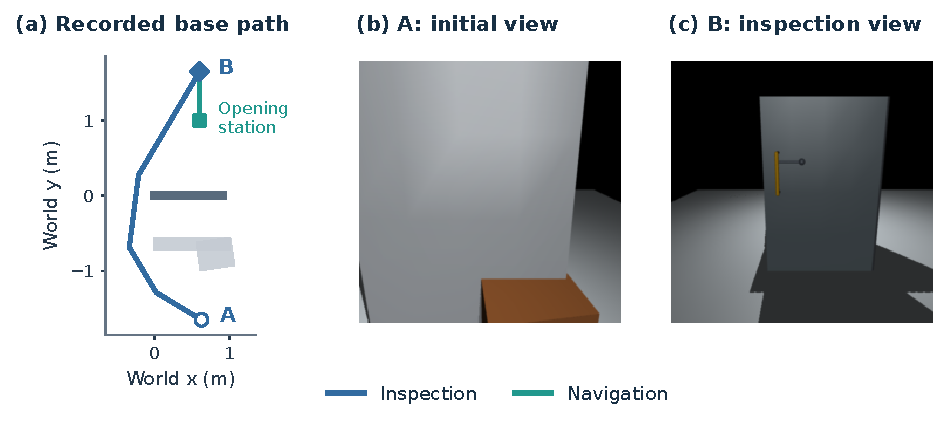
\includegraphics[width=\linewidth]{figures/methods/report_active_motion.pdf}
  \caption{Primary-policy replay from test cohort C. (a) Recorded base path with door and obstacle geometry in gray; viewpoints A and B correspond to (b) the initial view and (c) the reached inspection view. The base then reaches the opening station and opens the door. The episode covers 4.62~m in 61.99 simulated seconds.}
  \label{fig:active_motion}
\end{figure}

\fi

% !TeX root = ../../main.tex
\subsection{Physical Data Generation}
For each scene, we execute both direct and inspection branches, four stations,
and two grasp candidates, yielding $2\times4\times2=16$ physical candidate
records. Each trial has its own initialized episode and a continuous execution
prefix. A record stores scene/group identity, branch, station and grasp IDs,
initial and reached RGB-D, robot state, terminal outcome, failure stage, and
measured inspection distance and duration. The success predicate in
Section~\ref{sec:setup} generates outcome labels. All successes and failures
remain in the dataset; unavailable grasp observations are masked in G's
training loss. Complete parameter groups stay within one split, and
normalization is fitted on training data.

% !TeX root = ../../main.tex
\begin{samepage}
\subsection{Downstream Supervision for Positioning and Grasping}
P and G predict probabilities for success, other failure, and collision. We
score their outputs by expected terminal utility,
\begin{equation}
 V=\sum_c p(c)u_c,\qquad
 u=(1,-1,-1-\rho,0),
 \label{eq:utility}
\end{equation}
where the fourth entry denotes refusal and $\rho=1$ at deployment. P masks
excluded stations and appends a zero-valued refusal action. The heads are
trained by class cross-entropy.
\end{samepage}

Let $C_{s,b,p,g}$ be the recorded outcome of grasp $g$ at station $p$ in
branch $b$ of scene $s$. G learns these candidate outcomes directly. P's target
uses the grasp that the current G policy selects:
\begin{equation}
 \hat g_{s,b,p}=\arg\max_g V_G(s,b,p,g),\qquad
 y_P(s,b,p)=C_{s,b,p,\hat g_{s,b,p}}.
 \label{eq:pg_target}
\end{equation}
This makes the supervision reflect the deployed continuation. For example,
if only the second grasp succeeds but G selects the first, P receives the
first grasp's failure label for that station. Improving G can subsequently
change P's target.

For each branch, the objective is P cross-entropy plus $0.5$ times the
cross-entropy of visible G records. The two branch losses are summed, with
unsafe post-inspection P decisions masked. Targets refresh every 40 updates
using training predictions. The chosen IDs and outcome-table lookups form
detached labels. Encoder LoRA and P/G heads update together while the original
H-JEPA core stays frozen.

% !TeX root = ../../main.tex
\subsection{Learning When to Inspect}
After selecting P/G, we freeze the continuation and compare its actual choices
in the two physical branches. The measured inspection advantage is
\begin{equation}
 A=U_{\mathrm{inspect}}-C-U_{\mathrm{direct}},\qquad
 C=0.2\frac{d}{6}+0.1\frac{t}{60},
 \label{eq:advantage}
\end{equation}
where $d$ is inspection travel in meters and $t$ is inspection duration in
simulated seconds. Both utilities come from the frozen policy's selected
actions. I receives initial-view features, the relative inspection command,
declared risk, and initial depth features. It predicts four outcome logits
and a nonnegative softplus cost, giving a net value
$\widehat V_I=\sum_c p_I(c)u_c-\widehat C$.

The joint inspection objective combines outcome classification, cost fitting,
and a decision term weighted by the magnitude of the measured advantage. With
$z_s=(\widehat V_{I,s}-\widehat V_{D,s})/0.2$, it is
\begin{align}
 \mathcal L_I&=\mathcal L_{\mathrm{CE}}
 +0.5\mathcal L_{\mathrm{MSE}}(\widehat C,C)+\mathcal L_{\mathrm{regret}},\\
 \mathcal L_{\mathrm{regret}}&=
 \frac{\sum_s w_s\,\mathrm{BCEWithLogits}
 (z_s,\mathbf 1[A_s>0])}
 {\max(\sum_s w_s,10^{-8})},\quad w_s=|A_s|e_s.
 \label{eq:regret}
\end{align}
Here $\widehat V_D$ is the frozen direct branch's predicted best value and
$e_s$ marks eligibility under the initial station mask. The decision term
emphasizes inspection errors with greater downstream cost. At runtime, I
compares its predicted net value with the best permitted station/refusal
value. The executor immediately refuses if the initial mask excludes every
station. Future observations and measured branch outcomes supply training
targets; inference uses the currently available view.

% !TeX root = ../../main.tex
\subsection{Training Stages and Checkpoint Selection}
The continuation experiments start from the validation-selected partial-map
P/G checkpoint, inherited from an earlier outcome-supervised mobile policy.
This two-level H-JEPA model already contains rank-8 LoRA and P/G outcome heads
adapted to simulated door opening. We resume the adapters with scaling $\alpha=16$ and
dropout 0.05 \citep{hu2021lora}. Table~\ref{tab:training} gives the latest
continuation budget. AdamW uses weight decay 0.01 and gradient clipping at 1;
P/G training uses BF16 autocast. Groups contain four related layouts, and the
paired sampler draws two different layouts from one training group per update.

\begin{table}[H]
\caption{Latest continuation settings. Learning rates are for the standard arm;
the low-rate controls multiply both P/G-stage rates by 0.1.}
\label{tab:training}
\centering\small
\begin{tabularx}{\linewidth}{@{}lXXX@{}}
\toprule
Stage & Trainable parameters & Updates and batch & Learning rate \\
\midrule
P/G & Existing LoRA and P/G heads & 320; 2 scenes; target refresh every 40
 & Heads \mbox{$3\times10^{-4}$}\newline LoRA \mbox{$2\times10^{-5}$} \\
I & Inspection head & 1600; up to 32 training rows & $3\times10^{-4}$ \\
\bottomrule
\end{tabularx}
\end{table}

P/G checkpoint selection compares direct and always-inspect validation
branches: fewer collisions first, then inspected-branch correctness, direct
correctness, total openings, net utility, and path length. Strict improvement
retains the earlier checkpoint on ties. We then freeze all non-I parameters
and select I using validation task outcomes and cost. Python, NumPy, Torch,
and CUDA use seed 42.

